\chapter{Complexity Factors}
\label{ch:unmaintainability}

After analysing the different approaches taken by previous work, we define a number of requirements and challenges our solution has to meet and overcome. Most of these generate complexity in the system, and make for potential issues for long term support of such a system. As such, starting with the analysis of these issues, we focus our attention on the maintainability issues related with this project.

\section{Generality}
\label{sec:complexity-generality}

To lower the coupling between our software and \acrshort{vtk}, we want it to be version-agnostic. This coupling is already weakened by the fact the library is developed to be backwards-compatible and the only major change to the API that broke this, happened between versions 4 and 6 of the library\footnote{\url{https://vtk.org/Wiki/VTK/VTK\_6\_Migration/Overview}.}. 

We also aim at enabling the user to exploit the library to its full potential, limiting the components that cannot be reached from within the development environment, and that require technical knowledge to be integrated through code. As we discussed in Section~\ref{sec:related-work}, both the OculusVTK implementation by Dreuning and the ActiViz plugin have this capability. The first is, however, limited to Python and using OculusVR supported \acrshort{hmd}s, whereas the second is limited by its performances. 

Hardcoding \acrshort{vtk}s features would make for the best performances, but would make the system plugin a huge collection of functions, as it would be necessary to wrap the calls for every class and method accessible to the user. This approach would potentially be the more performant, but hardly makes for a maintainable system.

Instead, our approach aims to integrate Dreuning's Python introspection scripts within a C++ native plugin, as this would still allow for a performing system written in C++ to access Python's capabilities when it is necessary to expose parts of \acrshort{vtk} the system has no direct access to.

Introducing these Python scripts within the C++ plugin can be achieved through two different approaches: keeping the Python component separate and make it communicate with the C++ native plugin or embedding the Python interpreter within the C++ code itself. 

Although the first option would make for better separation of concerns, it introduces a non-trivial issue with memory sharing, synchronization, and performance. As the two parts would need to communicate, both should be able to read and write the \acrshort{vtk} objects being handled while keeping execution time as low as possible. Although, these operations can achieve the required performances of completing a full cycle in around 11.1 ms (90 \acrshort{fps} for most \acrshort{hmd}s is the recommended refresh rate), comprising of updating both lenses' views, they require careful crafting and optimizing, introducing design and code complexities.

On the other hand, the embedding of the Python interpreter is a common choice and is discussed in the official guidelines of Python itself\footnote{\url{https://docs.python.org/3/extending/embedding.html}} and can achieve decent performances. In order to determine the overhead introduced by the embedding, we compare the execution times of an embedded application with the same application in pure Python and repeat this for direct access to \acrshort{vtk} and using the Dreuning's introspection scripts.s

The application we run is a stream tracer of a density dataset for \acrshort{vtk} applications. The final visualization is composed of the outline and the streamlines. The pipeline can be seen in Figure~\ref{fig:streamtracer_pipeline}. This pipeline has been implemented in Python 3.7 directly using the \acrshort{vtk} library and accessing it through a modified and expanded version of Dreuning's scripts, the embedded verion of the Python interpreter in C++ executing Python calls directly to \acrshort{vtk}, and finally again through C++ by calling the functionality exposed by the modified Dreuning's scripts. The code for each of these tests is presented in Appendix~\ref{apx:streamtracer-performance-tests} and the results are shown in Table~\ref{tab:streamtracer-performance-tests-results}.

\begin{figure}[ht!]
    \centering
    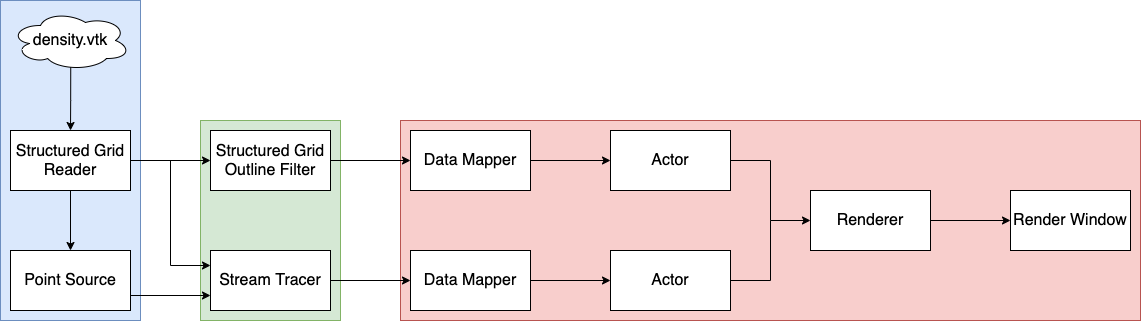
\includegraphics[width=\textwidth]{pictures/streamtracer_pipeline.png}
    \caption{VTK pipeline of a Stream Tracer on a density dataset.}
    \label{fig:streamtracer_pipeline}
\end{figure}


\begin{table}[ht!]
    \centering
    \begin{tabular}{lllll}
    \hline
    \multicolumn{1}{c}{\multirow{2}{*}{\textbf{Operations}}} &
      \multicolumn{2}{c}{\textbf{Python}} &
      \multicolumn{2}{c}{\textbf{C++}} \\ 
    \multicolumn{1}{c}{} &
      \multicolumn{1}{c}{\textbf{Native}} &
      \multicolumn{1}{c}{\textbf{Introspection}} &
      \multicolumn{1}{c}{\textbf{Native}} &
      \multicolumn{1}{c}{\textbf{Introspection}} \\ \hhline{=====}
    Loading*                       & \multicolumn{1}{l}{0}         & 1.8973614 & 0.7491320 & 2.7688682 \\
    Object instantiation**         & \multicolumn{1}{l}{0.0046789} & 0.0001833 & 0.0000791 & 0.0001782 \\
    Reader update                  & \multicolumn{1}{l}{0.5265901} & 0.5276741 & 0.0000029 & 0.2713980 \\
    Attribute setting**            & \multicolumn{1}{l}{0.0000045} & 0.0000104 & 0.0000038 & 0.0000119 \\
    Attribute getting**            & \multicolumn{1}{l}{0.0000517} & 0.0000524 & 0.0000011 & 0.0000938 \\
    Set connection**               & \multicolumn{1}{l}{0.0000131} & 0.0000086 & 0.0000018 & 0.0000139 \\
    Finalizing*                    & \multicolumn{1}{l}{0}         & 0         & 0.0196236 & 0.0258235 \\ \hline
    Total execution time           & \multicolumn{1}{l}{0.5525628} & 2.4283721 & 0.7691996 & 3.0672562 \\ \hline
    Execution time without loading & \multicolumn{1}{l}{0.5525628} & 0.5310107 & 0.0004440 & 0.2725645 \\ \hline
    \end{tabular}
    \caption{Performance test results on Python and C++ using VTK with and without introspection.\\
    *: time required within the execution to load the necessary structures for embedding Python and using the Introspector.\\
    **: average times calculated on the different methods used within the code.}
    \label{tab:streamtracer-performance-tests-results}
\end{table}

As shwon in by the results, the best solution for overall execution would be a native written Python software. However, stripping the execution time of the one-time loading and finalizing delays, the execution of the native and introspective versions of the algorithm take virtually the same time. What is more surprising, is the 50.68\% faster execution of the C++ introspective application using an embedded Python interpreter. The native C++ version using the embedded Python interpreter to call \acrshort{vtk} natively in Python shows the best performances as the only real time spent executing code is the loading of the Python interpreter and its finalizing.

As such, to both accomodate our requirement of generality and performance, we see the embedding of the Python interpreter into the C++ native plugin for Unity and leveraging of the Python introspective capabilities as a good candidate for our implementation. However, taken into account the performances that C++ can achieve, and to further give expert users the possibility to levarage the languages strongsuits, we incorporate in our design of the system a component that allows the user to write custom code that can be easily added to the plugin to run natively some code.

\section{Memory Sharing}

The choice of the embedding of the Python interpreter also stems from a second consideration: one of the main issues of trying to introduce introspection capabilities to C++ is its memory handling. First of all, introducing these capabilities to C++ is not a straight forward task, as it has already been studied in the past. In particular, non-intrusive solutions that do not require modifications to the compiler introduce memory overheads \cite{bayser2012rtti} and/or without exposing complete introspection systems, as constructs such as \verb|union| cannot be easily handled \cite{tyng1998nonintrusive}.

Using solutions that would modify the C++ compiler are also not of our interest as they introduce a very tight coupling with the modificiations in place, and potential for unexpected breaking points down the development process that would not be easily traceable back to these modifications. For these reasons we see these solutions as non-starters for our project.

As such, we can introduce these capabilities into our solution not through the use of C++ alone, but using languages such as Java or, indeed, Python that do have them natively. This though presents a challenge in how this component would communicate with the C++ one. If the components were to be separate, we would need to either synchronize their data at every call through protocolized communication or we would have to create shared memory areas where the shared objects would be instantiated.

As we are using Python as our language, and it has a native API to embed it within C and C++, this is a non-issue for us, as the memory are of the interpreter is a subset of the program's memory area, and as such C++ can easily pass wrapped objects to Python without having to create shared memory areas or caring for synchronization and protocols.

For even further support, \acrshort{vtk} ships with a module for facilitate Python/C++ integrations exposing functions that easily wrap C++ and unwrap Python \acrshort{vtk} objects, as each wrapped Python object keeps a reference to the C++ object, and from the pointer to the object the wrapper can be generated.

\section{Python Embedding}

As the developers of Python already forsaw a use for Python tightly coupled with other languages, as well as the possibility for users to extend the language, the interpreter can be embedded using natively supported calls that are part of what is called the Python/C API \cite{python_c_api}. This API gives access to the ability to instantiate a Python interpreter within a C/C++ software that shares with the interpreter its memory, in order to allow both to access data in a fast and controlled manner.

However, this API is verbose, escpecially while working with objects, which made us consider the usage of a third party library called Boost::Python
%TODO: devi mettere la ref? come devi formattare i nomi di cose registrate?
, which extends the Python/C API, further simplifying the embedding of the interpreter. The most useful feature which would immensily aid the maintainability and readability of our code is its automatic handling of the Python reference count of objects.

In order for Python's garbage collector to properly dispose of an object, the language decorates each instance with a reference count, which is a counter that keeps track of how many variables are referencing the object. Once this counter reaches zero, the garbage collector disposes of it and frees its memory. The Python/C API leaves the handling of these counters to the user through the usage of \verb|Py_DECREF| and \verb|Py_INCREF| macros.

While this freedom allows for more sophisticated uses of the interface, it also makes the code more complex to read, making the codebase larger in terms of SLOCs and more complex as it requires controlling references and being careful not to create memory leaks. This is made more complicated as some functions of the API increase the reference count while others \textit{steal} its reference from the caller, making the system prone to memory leaks. This is somewhat helped by the introduction of the \verb|Py_XDECREF| macro which decreases if not null or already zero.

On the other hand, while Boost::Python aids in making the code more readable and maintainble, it also introduces a further coupling with a third party library, which is comprised of a multitude of functionality that is not required for our software, introducing breaking points. Furthermore, the structures wrapped around \verb|PyObject|, the controls and the exception handling system introduced by the library results in overhead on both memory and speed of the execution, which is not ideal in our performance-critical environment. 

%TODO:Should I leave this here or move it to Future work?
As a proof of concept, to showcase the capabilities of our system, we do not use Boost::Python, so to limit external coupling and overheads. We recognise though that the advantages of the library are not trivial and it should be explored as a potential option for future updates to the project.

\section{Unity Integration}

The foremost factor of complexity and maintainability issues is the integration of the system with the Unity Engine. Integrating two rendering components is challenging in two main ways. First to tackle is the issue of sharing resources and the rendering context, as taken separately Unity and \acrshort{vtk} have both their own objects, memory spaces and rendering contexts.

To simplify the issue, we can make our solution a part of the Unity environment we are developing by creating a Unity native plugin. These are libraries written in C, C++ or Objective-C that are not constrained by the Unity environment like C\# Managed plugins \cite{technologies_21AD}. By making our solution a Unity native plugin, we now have to solve the problem of sharing data between the rendering contexts of Unity and \acrshort{vtk}.

As we are taking a similar approach to Wheeler et al.'s, we also follow their solution to solve this issue. In VtkToUnity the sharing of resources between the two rendering contexts is achieved using OpenGL Core ES technology, as it allows for sharing some objects between OpenGL Core conforming contexts \cite{wheeler_virtual_2018}. As the specification of these contexts is forward compatible, we also do not need to worry about compatibility between versions \cite{khronos_opengl_2021}.

We use as base for our software Wheeler's VtkToUnity plugin, as such we use the same system they developed for sharing data between rendering context and for integrating the event loops of Unity and \acrshort{vtk}. This second issue was also tackled by Wheeler et al. by nesting the \acrshort{vtk} event loop iteration in Unity's using the engine's event queue event handlers and graphics callbacks \cite{wheeler_virtual_2018}. The obtained architecture for the plugin is shwon in Figure~\ref{fig:wheeler-architecture}. Most of the functionality handling these loops is implemented in the C\# scripts of Unity, which call the correct native function from the plugin in order to trigger the corresponding event in \acrshort{vtk}. A zoom in of the architectural specification can be seen in Figure~\ref{fig:wheeler-architecture-zoomin} where the particular calls from the scripts is highlighted and what is called in \acrshort{vtk} as a consequence for a particular Unity scene developed by Wheeler et al. \cite{wheeler_virtual_2018}.

\begin{figure}[ht!]
    \centering
    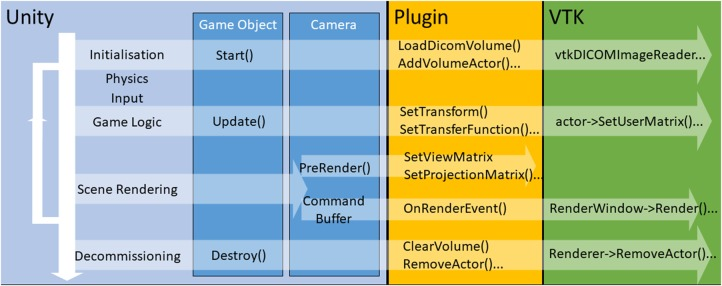
\includegraphics[width=\textwidth]{pictures/wheeler_architecture_zoomin.jpg}
    \caption{Wheeler et al.'s script handling of the VTK event loop.}
    \label{fig:wheeler-architecture-zoomin}
\end{figure}

